\chapter{Analysis}

\section{Introduction}

\subsection{Client Identification}
My client is Judy Rust. She is an ex-social worker who now owns and operates a charity shop known as Rusty Scraps in Hertfordshire. Judy opened her shop in 2012, after having worked with child fostering programs for 21 years. She isn't particularly computer literate, only using a basic ACER laptop to socialize and shop online. Judy wishes that she can improve her computer abilities to be able to improve her business's organisation and efficiency, as well as to be able to complete more activities on her laptop instead of having to rely on less efficient methods.
\subsection{Define the current system}
Judy's shop current employs a physical write-up on paper system for when somebody donates an item to the shop to be sold. Since Judy owns the shop and is not part of a charity, she has created and implemented the system herself. The item is first inspected by whatever staff is at the counter at the time, where they will do a very brief examination as to if the item is in a donation-quality condition. If the item is of not of that quality condition, it is refused. If it is however able to be donated, the member of staff quickly writes a brief description of the item on a sheet of notepad paper (this paper goes on to become the item 'tag'), and ask the donator to sign the paper with their name, address and contact number, the date of the current day, and finally their signature, relinquishing their ownership of the item and thus transferring it to the business. The employee who dealt with that transaction also puts their initials on the paper too (. This paper is attached to the item with a piece of adhesive tape.
The item is then transferred to the store room in the back to be evaluated a second time for quality, then priced and finally sorted into system of other items (so similar items would be placed together (i.e. a chair and a sofa would go together as they are both "Furniture")). The item is then eventually placed into the shop front to be sold to the public. When the item is placed, the paper containing the donator's information and item description is placed upon a pile of similar papers that have the same thing written on them, for all the items able to be purchased in the store front. When an item is bought, the paper of that item is then transferred to a safe box of "Receipts". All receipts collected during the day are checked against the amount of money in the till to make sure all financial transactions were correct.

\subsection{Describe the problems}
Judy has explained the efficiency problems of the system along with personal issues with it. The most apparent issue is the record keeping, where there seems to be a potential lack of consistency, security and organisation. When it comes to organization, paper slips are often misplaced or discarded as they give the appearance of being useless

Another problem is record keeping, as there is very little security on the shop's transaction history. The lockbox containing all previous transactions could easily be picked up and taken, leaving the shop without a backup. Another issue is the current item categorizing system. So far, items are only paired together when it's convenient, and the categories are made up on the stop instead of having a predetermined list of ways to categorize items. The current system leads to a much unorganized and potentially confusing store room. Another problem is the paper records. Judy herself and all of her employees have reported their dislike of the paper system they use, citing that it is tedious and confusing sometimes. An electronic system would play to everyone's benefits.
\subsection{Section appendix}

\begin{figure}[H]
    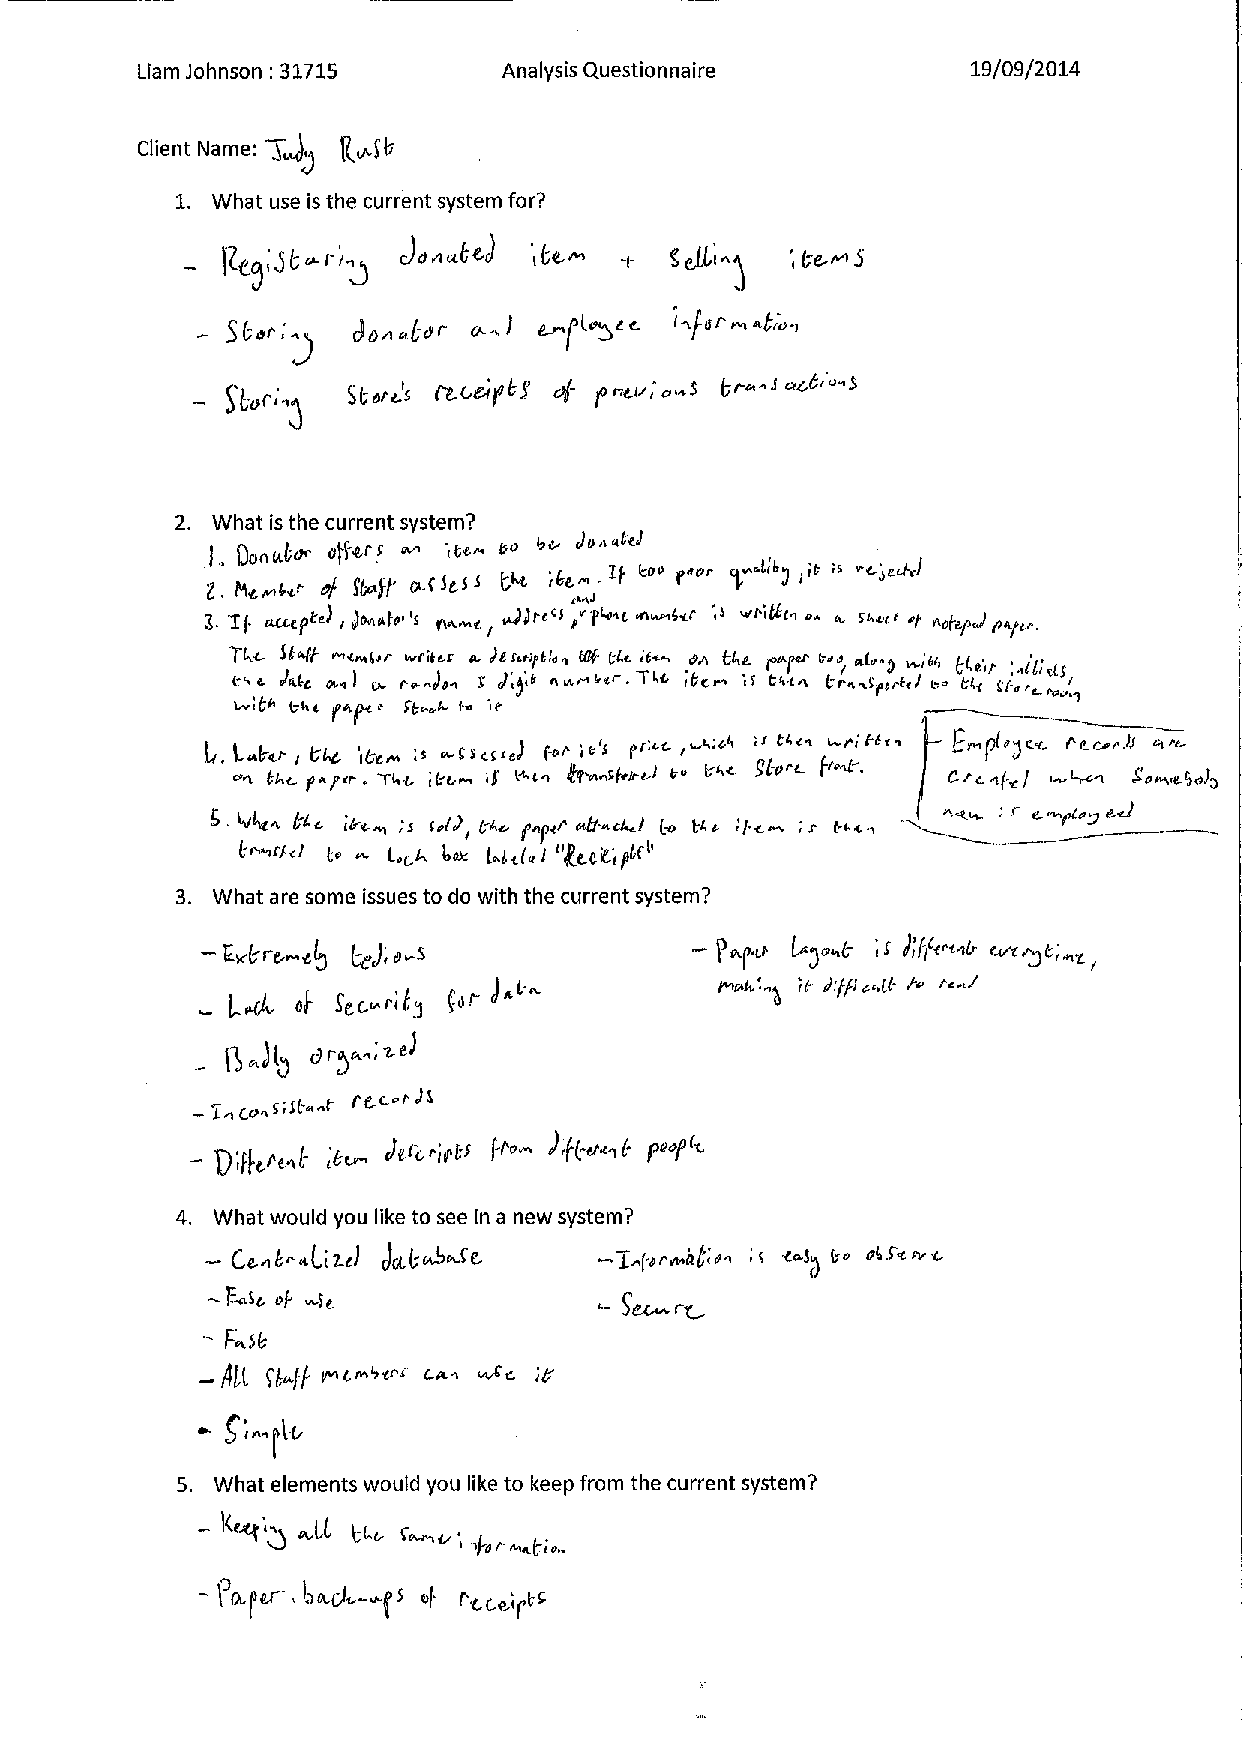
\includegraphics[width=\textwidth]{Appendix1.pdf}
    \caption{Questionnaire from the interview Page 1} \label{fig:SectionAppendix}
\end{figure}

\begin{figure}[H]
    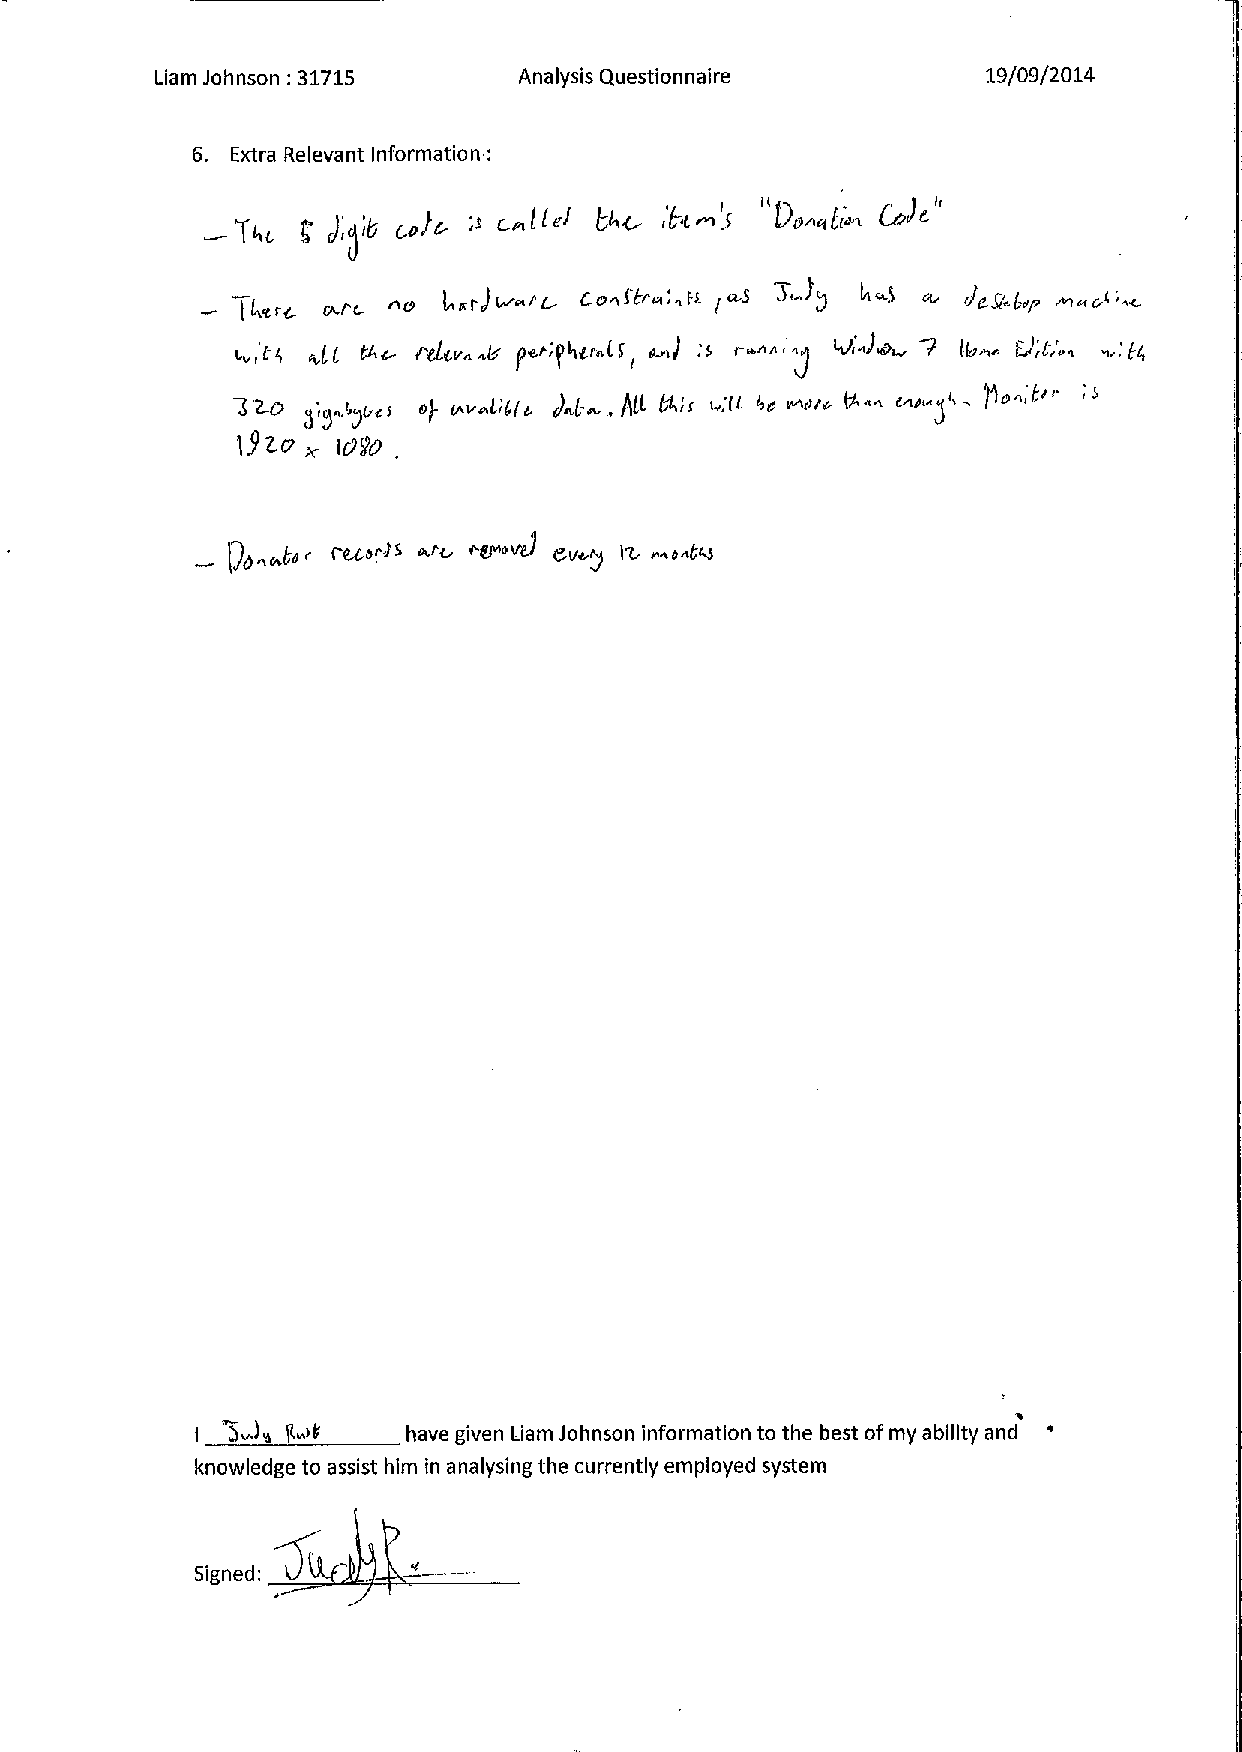
\includegraphics[width=\textwidth]{Appendix2.pdf}
    \caption{Questionnaire from the interview Page 2} \label{fig:SectionAppendix}
\end{figure}
\section{Investigation}

\subsection{The current system}

\subsubsection{Data sources and destinations}
The system that’s in place now uses these data sources: staff member, donator, and the item tag.
 Staff members information is currently kept in a paper based form in the private office of the shop. The data is stored on many different pieces of paper and each staff member has a paper folder with all of their own information in it. This information has the details of their name, home address, postal code and contact number(s). The details for their payment are more organized and are secured in a metal filing cabinet with a lock. This cabinet is not large enough to contain the employee information and their payment details. As mentioned before, a donator will leave their information with the member of staff, and these details get attached to the item before sale, and then removed and (badly) secured after sale.

\begin{tabular}{|p{3cm}|p{4cm}|p{4cm}|p{2cm}|}
	\hline
	\textbf{Data Source} & \textbf{Attributes} & \textbf{Example} & \textbf{Destination}\\ \hline 
	\textbf{Staff Member} & \textbf{Initials, Donation Code, Item Description} & \textbf{JJ, 71723, “A fridge”} & \textbf{Item Tag}\\ \hline
	\textbf{Donator} & \textbf{Name, Address, Contact Number(s), Item(s) of Donation} & \textbf{Johny Johnson, 7 Rinnocks Close, Herts, SY5 9CX, 0700502340, A vase and a flower} & \textbf{Item Tag} \\ \hline
	\textbf{Staff Member} & \textbf{Item price} & \textbf{£4.20} & \textbf{Item Tag} \\ \hline
	\textbf{Item} & \textbf{Notepad Data} & \textbf{“JJ, 71723, A fridge, £4.20”} & \textbf{Receipt Box} \\ \hline
\end{tabular}

\subsubsection{Algorithms}
The algorithm used in the process  of donation are fairly simple and often tedious, as it must be repeated every time a new item is brought in.

\begin{algorithm}[H]
    \caption{Check if the item can be donated}
\begin{algorithmic}[1]
\If{$"donated\_item.quality" <"minimum\_donation\_quality"$}
\Function{Refuse}{donated\_item}\EndFunction
\Else
\State $item\_tag.donator\_info \gets  donator\_information$
\State $item\_tag.staff\_info \gets  staff\_information$
\EndIf
\end{algorithmic}
\end{algorithm}

When the item is sold, the process is shown by this algorithm.

\begin{algorithm}[H]
	\caption{Process of sale}
\begin{algorithmic}[2]
\State $item.sold \gets False$
\While {$item.sold \neq True$}
\If {$Sale Requested For Item$}
\Function{SaleProcess}{item}\EndFunction
\If {$sale == True$}
\State $item.sold \gets True$
\Else 
\State $pass$
\EndIf
\Else 
\State $pass$
\EndIf
\EndWhile
\end{algorithmic}
\end{algorithm}


\subsubsection{Input Forms, Output Forms, Report Formats}
The only input form is the item tag in the current system. Here is a reproduction of an example item tag.

\begin{figure}[H]
    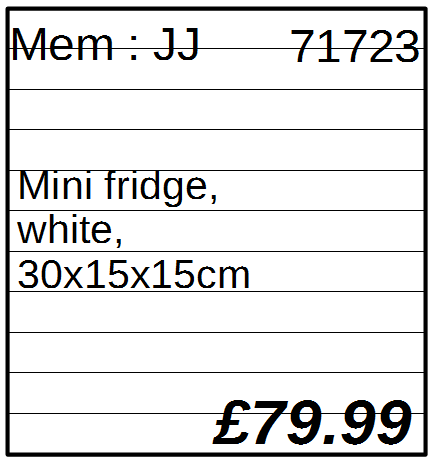
\includegraphics[width=\textwidth]{ExampleItemTag.png}
    \caption{A computer-based reproduction of item tag} \label{fig:ItemTag}
\end{figure}

\subsection{The proposed system}

\subsubsection{Data sources and destinations}
The proposed systems data flow will be very similar to the current system, in that the data will end up as a electronic version in the database instead of physically being written on paper.

\begin{tabular}{|p{3cm}|p{4cm}|p{4cm}|p{2cm}|}
	\hline
	\textbf{Data Source} & \textbf{Attributes} & \textbf{Example} & \textbf{Destination}\\ \hline 
	\textbf{Staff Member} & \textbf{Initials, Donation Code, Item Description} & \textbf{JJ, 71723, “A fridge”} & \textbf{Item Data}\\ \hline
	\textbf{Donator} & \textbf{Name, Address, Contact Number(s), Item(s) of Donation} & \textbf{Johny Johnson, 7 Rinnocks Close, Herts, SY5 9CX, 0700502340, A vase and a flower} & \textbf{Item Data} \\ \hline
	\textbf{Staff Member} & \textbf{Item price} & \textbf{£4.20} & \textbf{Item Data} \\ \hline
	\textbf{Item} & \textbf{Notepad Data} & \textbf{“JJ, 71723, A fridge, £4.20”} & \textbf{Item Data} \\ \hline
\end{tabular}

In the new system, instead of having this paper created, edited and then stored, all the data will be entered onto the database where it can be edited easily later.
 
\subsubsection{Data dictionary}
\begin{tabular}{|p{3.25cm}|p{1.5cm}|p{1.75cm}|p{3cm}|p{3.5cm}|}
\hline
\textbf {Data Name} & \textbf {Data Type} &\textbf {Character Length} &\textbf {Validation Type} &\textbf {Example} \\ \hline
\textbf {ItemDonationCode} & \textbf {String} &\textbf {5} &\textbf {Range Check} &\textbf {64832} \\ \hline
\textbf {ItemDescription} & \textbf {String} &\textbf {0 - 30} &\textbf {Range Check} &\textbf {“A leather chair”} \\ \hline
\textbf {ItemPrice} & \textbf {Float} &\textbf {0 - 6} &\textbf {Range Check, Type Check} &\textbf {42.56} \\ \hline
\textbf {ItemCategory} & \textbf {String} &\textbf {0 - 20} &\textbf {Range Check} &\textbf {“Furniture”} \\ \hline
\textbf {ItemQualityCheck} & \textbf {Boolean} &\textbf {} &\textbf {True/False} &\textbf {True} \\ \hline
\textbf {ItemSaleCheck} & \textbf {Boolean} &\textbf {} &\textbf {True/False} &\textbf {True} \\ \hline
\textbf {DonatorName} & \textbf {String} &\textbf {0 - 30} &\textbf {Range Check} &\textbf {“Wendy Hudden”} \\ \hline
\textbf {DonatorAddress1} & \textbf {String} &\textbf {0 - 20} &\textbf {Range Check} &\textbf {“2 Not Lane”} \\ \hline
\textbf {DonatorAddress2} & \textbf {String} &\textbf {0 - 20} &\textbf {Range Check} &\textbf {“Flat 20C”} \\ \hline
\textbf {DonatorCity} & \textbf {String} &\textbf {0 - 15} &\textbf {Range Check} &\textbf {“Melbreth”} \\ \hline
\textbf {DonatorCounty} & \textbf {String} &\textbf {0 - 15} &\textbf {Range Check} &\textbf {"Cambridgeshire"} \\ \hline
\textbf {DonatorPostCode} & \textbf {String} &\textbf {0 - 8} &\textbf {Range Check} &\textbf {“SG9 3KW”} \\ \hline
\textbf {DonatorContact} & \textbf {String} &\textbf {0 - 15} &\textbf {Range Check} &\textbf {“01189998235”} \\ \hline
\textbf {StaffName} & \textbf {String} &\textbf {0 - 30} &\textbf {Range Check} &\textbf {“Wiggy Wog”} \\ \hline
\textbf {StaffInitals} & \textbf {String} &\textbf {0 - 6} &\textbf {Range Check} &\textbf {“WW”} \\ \hline
\end{tabular}
\subsubsection{Volumetrics}
Judy has stated that the shop receives no more than 30 items a week. Looking at the Data Dictionary, an item has 15 fields for unique identification. Each field has no more than 30 characters filling it. Going by that ASCII uses 1 byte per character, we can calculate roughly how much data the database will max out at.

15 x 30 = 450

So that makes 450 bytes of data per item. Judy has said that she receives no more than 30 items in a week, so we can use 30 as a upper bound.

450 x 30 = 13500

That makes 13500 bytes of data recieved in a week. The records of items are kept for a year, then discarded due to the space they took up.

13500 x 52 = 702000

In a year then, there is at most 702000 bytes (only 0.702 Megabytes) of data that the system can possibly use. It is a tiny amount of data.Let’s assume that the program will take up no more than 5 Megabytes, given the need for an installation of Python and all the needed packages and modules.
That’s, in total, 5.70MB. A tiny amount of data. The problem Judy had was that keep records for so long took up a lot of physical space, meaning she had to discard some. Now, as the data is so small, she can keep years and years worth of data thanks to the digitization of the system.

\section{Objectives}

\subsection{General Objectives}
\begin{itemize}
    \item Create a much more efficient system for Judy than the currently existing one
    \item Create a easy to use system for Judy
\end{itemize}
\subsection{Specific Objectives}
\begin{itemize}
    \item Have the system be easy to understand
    \item Have the system be easy to use
    \item Have the system be reliable when storing records
	\item Have the system be secure as to comply with laws regarding data security
	\item Have the system be able to have multiple profiles for different people to use
	\item Have the system be tailored for the desired purpose
	\item Have the system store data in the suitable format
	\item Have the system be free of potential system-threating bugs and glitches
\end{itemize}
\subsection{Core Objectives}
\begin{itemize}
    \item Must be able to hold data about a donated item
    \item Must be able to have the data displayed by different attributes of each item
    \item Must be able to edit existing data
	\item Must be useful towards it's purpose
\end{itemize}

\section{ER Diagrams and Descriptions}

\subsection{ER Diagram}
\begin{figure}[H]
    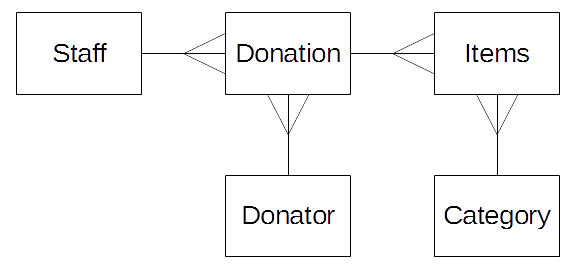
\includegraphics[width=\textwidth]{ERDiagram.png}
    \caption{ER Diagram showing item registration} \label{fig:ER Diagram}
\end{figure}
\subsection{Entity Descriptions}
Staff( \underline{StaffInitals},\textit{ItemDonationCode},StaffName)

Donator(\underline{DonatorName}, \textit{ItemDonationCode}, DonatorAddress1, DonatorAddress2, DonatorCity, DonatorCounty, DonatorPostCode, DonatorContact)

Item(\underline{ItemDonationCode}, \textit{StaffInitals}, \textit{DonatorName}, ItemDescription, ItemPrice, ItemCatagory, ItemQualityCheck, ItemSaleCheck)

\section{Object Analysis}

\subsection{Object Listing}
\begin{itemize}
    \item Staff Member
    \item Item
    \item Donator
\end{itemize}

\subsection{Relationship diagrams}
\begin{figure}[H]
    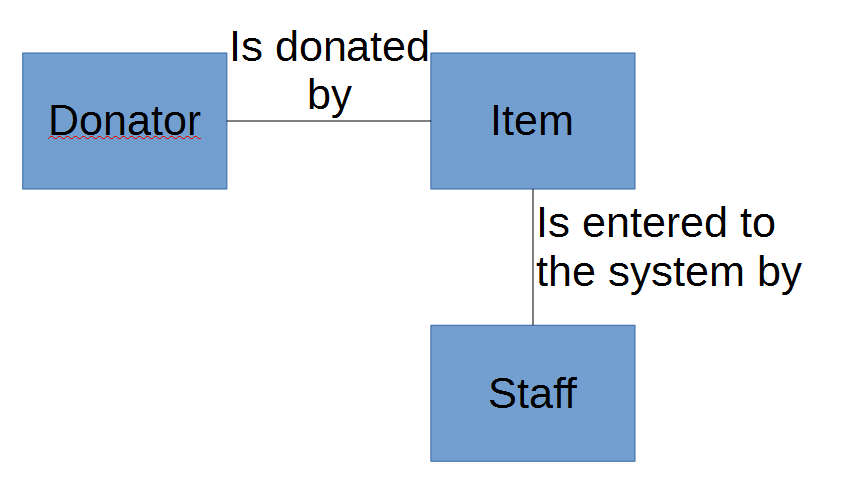
\includegraphics[width=\textwidth]{RelationshipDiagram.png}
    \caption{A relationship diagram of the objects} \label{fig:Relationship Diagram}
\end{figure}
\section{Constraints}

\subsection{Hardware}
A computer was donated to the shop last June. This computer is a Dell desktop computer, with 1080p monitor and accessories, running Windows 7 Home Edition. 8GBs of DDR3 RAM, an i5 Intel processor, and a AMD video card. Judy has said that she is perfectly happy to us this computer as a work PC, along with being able to work on it all day. Looking at a technical standpoint of the components, it is more than enough to satisfy whatever my program needs, as my program will take up very little processing power, and require very little storage space, for both the program data itself and the database.

\subsection{Software}
Windows 7 Home Edition does not limit what software can be made for Judy's specifications. She's used WindowsOS whenever she has used a desktop/laptop, so she would prefer for the OS to stay the same.

\subsection{Time}
Judy has stated that she has no need for the software to be completed in a time limit. Although, this does not mean I can take as much time as I like the the program and project overall, as the coursework has a set deadline from in April 2015 to be completed by and submitted.
\subsection{User Knowledge}
Judy, while regularly using a computer, describes herself as "not following everything that’s happening" she explains that she only really uses a laptop to surf the web, do online shopping and partake in social networking. While she has had to use Microsoft's Word and Excel programs during her previous employment, she claims to have 'never had a problem' with Word, but 'couldn't understand properly' how to use Excel. The databases she used during her last job apparently had "about 10 columns just to describe something like an address and far too many rows on screen to be able to focus on something specific". This kind of feedback reinforces that while the client has some IT skills, overall they are not completely computer literate can would only be able to use a program if it had a GUI and clear actions when interacting with it.

\subsection{Access restrictions}
The system will be accessible by Judy and all of the staff working at her shop. Each employee must change the 'current user' in the program to themselves while performing any actions with the program, as to make sure changes made to the database can be tracked to a the user, should an error be entered, the error can be traced back to the user at the time.

\section{Limitations}

\subsection{Areas which will not be included in computerisation}
In terms of record keeping, everything will be computerised, except for the secured employee records. These will not be converted digitally, as Judy would prefer to have those records not have a back-up, just for the sake of security.


\subsection{Areas considered for future computerisation}
Although the shop gets a steady stream of donations (20-30 items a week), there is plenty of storage space for a larger intake, so it could be worthwhile in the future to set up a website for the shop to get more donations and more business. By having the database connect to the website also, it would mean people could search the contents of the shop without having to be there, which is a very desirable quality with today’s shoppers. This would give the shop better representation and could evolve for the donation process to be done remotely at someone’s home and they can ship their items to the shop, instead of dropping in.

\section{Solutions}

\subsection{Alternative solutions}
    \begin{tabular}{|p{4cm}|p{4cm}|p{4cm}|}
	\hline
	\textbf{Solution} & \textbf{Advantage} & \textbf{Disadvantage} \\ \hline
	\textbf{Improve upon the current system} & \textbf{No vast overhaul will be required
System will be familiar to those who used it previously
Should be cheap and not too complex to achieve
} & \textbf{Underlying problems with the system may never be resolved
Would not improve efficiency very much
} \\ \hline
	\textbf{Database Management Software} & \textbf{Already exists
Will have technical support from creators
} & \textbf{Such software tends to be made for sale, instead of open-source, requiring a purchase.
Not that user friendly
Can take up significant amounts of hard drive space
} \\ \hline
	\textbf{Web Application} & \textbf{Will be accessible anywhere assuming there is a proper connection and equipment available
Web-based applications tend to be able to be embedded into other applications with relative ease
} & \textbf{Much higher security requirements
More web-based knowledge required to used
} \\ \hline
	\textbf{Spreadsheet software} & \textbf{Many programs already exist and are readily available
Judy herself has had experience with one before (Excel).
Generally doesn’t require that high of IT skills to understand and operate.
} & \textbf{Judy herself has expressive her annoyance of having to use such a software.
Not as user-friendly as required.
Such software tends to be made for sale, instead of open-source, requiring a purchase.
Can take up significant amounts of hard drive space
} \\ \hline
	\textbf{Custom Designed Python Program} & \textbf{Can be custom made to fit specifications
Custom GUI to fit the user’s specific needs
No purchase required
Shouldn’t be very resource intensive
} & \textbf{Will take time to develop
Software may not be able to be used in another circumstance except for the one it is designed for
Coding a GUI on top of a DBS is a lot of work
} \\ \hline
	\end{tabular}
\subsection{Justification of chosen solution}
The solution that will be used is 'Custom Designed Python Program' for the following reasons:
\begin{itemize}
    \item I know much about the Python language, and I could not create the same application using any other language
    \item All the aspects of the program will be made to fit Judy's requirements and specifications 
	\item A easy-to-understand GUI can be created, also to fit Judy's needs
	\item The program will not be very resource intensive on the computer it is run on, allowing it to be used on a variety of different machines if required
	\item The program and all the data are not likely to take up much space (20MB maximum) and it will be very easy to create backups of program versions or database copies from different dates
	\item This new system will be superior to the current system

\end{itemize}